% vim: set spell spelllang=en_gb tw=80:
\chapter{Preparation}

% \guidance{%
%   Principally, this chapter should \textbf{describe the work which was
%   undertaken before code was written}, hardware built or theories worked on. It
%   should \textbf{show how the project proposal was further refined and
%   clarified}, so that the Implementation stage could go smoothly rather than by
%   trial and error.\\
%   Throughout this chapter and indeed the whole dissertation, it is essential to
%   \textbf{demonstrate that a proper professional approach was employed}.\\
%   The nature of this chapter will vary greatly from one dissertation to another
%   but, underlining the professional approach, this chapter will very likely
%   include a \textbf{section headed “Requirements Analysis”} and
%   \textbf{incorporate other references to the techniques of Software
%   Engineering}.\\
%   The chapter will cite any \textbf{new programming languages and systems which
%   had to be learnt} and will \textbf{mention complicated theories or
%   algorithms} which required understanding.\\
%   It is essential to \textbf{declare the Starting Point} (see Section 7). This
%   states \textbf{any existing codebase or materials} that your project builds
%   on.  The text here \textbf{can commonly be identical to the text in your
%   proposal}, but it may \textbf{enlarge on it or report variations}. For
%   instance, the true starting point may have turned out to be different from
%   that declared in the proposal and \textbf{such discrepancies must be
%   explained}.
% }

\prechapter{%
  In this chapter, I will describe how I planned this project. I will start by
  mentioning the development methodology and tools I used. Following that, I
  will present and explain the requirements I used to guide the implementation
  of my project. From there, I will state my choice of technologies for this
  project. I will then go on to elaborate my starting point for this project.
  This will consist of a brief commentary on Coq, a comparison of existing tools
  that aim to help a user understand a Coq library and a description of Neo4j
  and some of its relevant plugins.
}

\section{Project Planning}

This project had two distinct phases: deciding how to model Coq proof-objects
(an exploratory phase) and applying network-analysis techniques (a technical
phase). For both, I chose a spiral software development model: think of an idea,
modify the code, propagate the necessary changes, evaluate the end-result and
repeat. This allowed me to experiment with ideas flexibly and easily.

I found Git (\href{http://git-scm.com}{\texttt{git-scm.com}}) and GitHub
(\href{http://github.com/dc-mak}{\texttt{github.com/dc-mak}}) invaluable during
this project; they allowed me to easily track, revert and review changes. I could
safely test new features on different branches before merging them and store
a copy of my work in multiple places. As it became apparent that precisely
specified versioning, build-dependencies and tests were useful in spotting
errors early, I added GitHub extensions such as
\href{https://travis-ci.org}{Travis-CI} for automated continuous-integration
builds.

\section{Requirements Analysis}

I developed and brought together several distinct components for
\emph{modelling} and translating (from Coq to the chosen model), displaying and
\emph{interacting} (Neo4j/Cypher) and \emph{computing} and analysing (plugins).
Below is a list of required features I used throughout development to guide and
provide context for implementation decisions.

\begin{itemize}

  \item \textbf{Modelling}: The model should
  \begin{enumerate}[label=\textbf{M\arabic*},ref={M\arabic*}]

    \item\label{req:m1} include as much relevant data as possible. Here,
      relevant means useful to understanding a large library, but not so much
      so as to obfuscate any information or make learning how to use the
      project more difficult.

    \item\label{req:m2} be flexible to work with and easy to translate. One
      could imagine different front-ends for interacting with and computing
      data from the model.

    \item\label{req:m3} strike a balance between size and pre-computing too much
      data. Figuring out which pieces of data can be reconstructed later and
      which are beneficial to compute during modelling will be a matter of
      experimentation and weighing up ease of implementation versus ease of
      later processing.

  \end{enumerate}

  \item \textbf{Interacting}: Interacting with the model should
  \begin{enumerate}[label=\textbf{I\arabic*},ref={I\arabic*}]

    \item\label{req:i1} primarily, allow users to understand the data. The
      following two points follow from this principal goal.

    \item\label{req:i2} support both graphical and textual modes of use. Small
      queries and novice users are likely to benefit from the presence of a
      well-designed GUI\@. However, larger queries requiring more computation
      and flexibility will benefit from a traditional, shell-like interface.

    \item\label{req:i3} be interactive and extensible. A static presentation of
      data, even in a GUI, would fail to make full use of graph-databases and
      the ability to query, in whatever way the user desires, information
      dynamically.

  \end{enumerate}

  \item \textbf {Computing}: Working with the model's data should
  \begin{enumerate}[label=\textbf{C\arabic*},ref={C\arabic*}]

    \item\label{req:c1} be enabled by a core library of good defaults. Certain,
      common functions should be ready `out-of-the-box' and provide users all
      they need to get started.

    \item\label{req:c2} allow the user to add their own functions. It is not
      possible to imagine and implement all the functionality users may desire
      and so it would be very useful to have a way to extend this project to suit
      their needs.

  \end{enumerate}


\end{itemize}

\section{Technologies Used}

Choice of implementation languages was, although an important decision, almost
completely dictated by the programs at the core of the project (Coq and Neo4j).

Coq and its plugins are written in OCaml
(\href{http://ocaml.org}{\texttt{ocaml.org}}); I stuck with it for two reasons.
First, it is almost always wiser to work with and modify existing systems (e.g.\
integrating with the build-system) and more representative of real-world work.
Second, as a functional language, OCaml benefits from a strong, static (and
inferred) type-system (which allows for easy experimentation and greater
confidence in correctness). Hence, using OCaml for other parts of the tool which
need not necessarily be in OCaml (e.g.\ the \texttt{dpd2} utility) was a welcome
and easy decision. OCaml has several other benefits too, such as
inductively-defined datatypes (useful for working with Coq's grammar) and good
editing tools.

Similarly, Neo4j and its plugins are (usually) written in Java, but several
languages are supported for the latter, both by Neo4j officially and by the
community. As I will explain in Section~\ref{sec:neo4j}, I found R to be the
most suitable for achieving this project's goals.

\section{Starting Point}

Both Coq and Neo4j have a rich ecosystem of tools and libraries built for them.
I examined the current landscape in detail to determine the software available
and see if I could use any of them as a starting point.

\section{Coq Proof-Assistant}

The Coq proof-assistant, implemented in OCaml, can be viewed as both a system of
logic -- in which case it is a realisation of the \emph{Calculus of Inductive
Constructions} -- and as a \emph{dependently-typed} programming language. Its
power and development are therefore most-suited and often geared towards
\emph{large-scale} developments.

On the logical side, Coq lays claim to feats of modern software-engineering such
as the Four-Colour Theorem~\cite{gonthier2008formal} (60,000 lines) and the
aforementioned \emph{Feit-Thompson} theorem (approximately 170,000 lines, 15,000
definitions and 4,200 theorems).

On the programming language side, Coq has served as the basis for many equally
impressive projects. The \emph{CompCert Verified C
Compiler}~\cite{leroy2012compcert} demonstrates the practical applications of
theorem-proving and dependently-typed programming by implementing and proving
correct an optimising compiler for the C programming language.
\emph{DeepSpec}~\cite{pierce2016science}, a recently announced meta-project,
aims to integrate several large projects such as \emph{CertiKOS} (operating
system kernels), \emph{Kami} (hardware), \emph{Vellvm} (verifying LLVM) and many
more in the hopes to provide complete, \emph{end-to-end} verification of
real-world systems.

Coq is a \emph{huge} project, developed by INRIA (France), and its size and
complexity are best experienced through untangling the source code for oneself.
Just for the implementation of the system (not including the standard library),
Coq features approximately 3 major ASTs, 6 transformations between them, 3000
visible types, 9000 APIs and 521 implementation files containing 228,000 lines
of dense, functional OCaml.

However, most of this massive project is sporadically (and tersely) documented.
Even after I received some guidance via the Coq developers' mailing-list, I
spent several hours browsing the source code trying to understand how the system
worked. Although I had some prior familiarity with \emph{using} Coq (as an
introduction to tactical theorem-proving and dependently-typed programming), it
was not useful for understanding the internals beyond context and how to compile
and use programs and libraries. However, it did serve as invaluable insight for
designing the model during the implementation phase.

\section{Existing Tools for Coq}\label{prep:coqtools}

There are many tools for Coq that, like my project, \emph{aim to help a user
understand a library}. I studied several to learn their approaches and analyse
their strengths and weakness. What follows is a detailed account of each tool
and why it did not meet this project's aims and requirements.

\subsection{Coqdoc}

Coqdoc is a documentation tool for Coq projects, included as part of the Coq
system. It can output to raw text, HTML, \LaTeX~and a few other formats to help
a user navigate and understand a Coq library.  Although it supports prettifying
code with syntax highlighting and Unicode characters, its most relevant feature
was its hyperlinking: potentially useful for building dependency graphs.

However, the whole tool works on an entirely \emph{lexical} level, with no
formal parsing or understanding of the code structure. Hence, since coqdoc could
not meet any of the modelling requirements (completeness~\ref{req:m1},
flexibility~\ref{req:m2} and size/pre-computation~\ref{req:m3}) I did not use
it.

\subsection{Coqdep}

Coqdep is a utility included with Coq that helps users understand a Coq
library's \emph{module-level} dependencies by tracking {\tt Require} and {\tt
Import} statements.  Although on first impressions, this tool seemed to offer
more flexibility than coqdoc, it was even more restrictive: it simply searches
for keywords (such as \texttt{Require} or \texttt{Import} for Coq  and
\texttt{open} or dot-notation module usage for OCaml) per file and outputs them
accordingly. As with coqdoc (and for the same reasons), I did not use coqdep
either.

\subsection{CoqSerAPI}

\emph{Coq Serialized (S-expression) API}
(\href{http://github.com/ejgallego/coq-serapi}{\texttt{github.com/ejgallego/coq-serapi}})
is a new library and communication protocol aiming to make low-level
interactions easier (using OCaml datatypes and s-expressions), particularly for
tool/IDE developers. It has a starting point for gathering some statistics on
proof-objects in a project. While this is likely to be useful in the future, it
is still far from complete and is more geared towards interactive
\emph{construction} (via a tool/IDE) rather than \emph{analysis}. As such,
tracking dependencies (critical to the modelling requirements) is not possible.

\subsection{dpdgraph}

dpdgraph
(\href{http://github.com/Karmaki/coq-dpdgraph}{\texttt{github.com/Karmaki/coq-dpdgraph}})
is a project which helps users understand the dependencies between proof-objects
in a Coq library. It does so by extracting information from compiled Coq
object-files to a \texttt{.dpd} file. It includes two example tools:
\texttt{dpd2dot} (for producing a \texttt{.dot} file for static visualisation)
and \texttt{dpdusage} (for finding unused definitions). Its developers intended
it to be a starting point for other tools to build upon.

Although lots of information such as notation, the relationship between
constructors and the types they construct, proof tactics, the precise kind of an
object (e.g.\  fixpoint, class, lemma, theorem, etc.) and which module an object
belongs to was missing, I thought it unlikely that the information was not
present in the compiled object files (since they are necessary for
term-construction and type-checking).

So, assuming the data was already present in those files, but simply
\emph{ignored or unused}, I focused on understanding and augmenting dpdgraph to
add the missing pieces to the model and output it to comma-separated values
(henceforth referred to as CSVs).

\subsection{Comparison}\label{subsec:comparison}

I have just discussed the many existing tools for Coq that \emph{aim to help a
user understand a library}. Table~\ref{table:features1} summarises the main
features of each. The features chosen reflect the strengths of each tool
and are justified and elaborated upon below. 

Bundle with Coq, coqdoc produces \textbf{hyperlinked source code} meaning
details such as \textbf{precise kinds} of a proof-object, \textbf{constructors
of a type} and \textbf{type-signatures} are immediately visible; hence those
five dimensions were included.  Also included in a Coq system is coqdep: a tool
for modelling \textbf{module-level dependencies} that can output a \texttt{dot}
file to present the dependencies \textbf{graphically}.

Coq Serialised (S-expression) API is an \textbf{interactive} IDE communication
protocol with facilities for gathering some basic \textbf{statistics}. Here,
interactive is used to mean that information is not presented all at-once,
\emph{statically}, but can instead be queried dynamically at run-time. An
example of a static display is Figure~\ref{fig:static}; it shows a medium-sized
Coq library as output by dpdgraph.

In principle, coqdep and dpdgraph can also support some degree of interactivity,
with support from other tools (which translate \texttt{.dot} files to
interactive JavaScript), although this is rarely done.  Lastly, dpdgraph models
\textbf{object dependencies} well, with some scope for distinguishing precise
kinds and displaying information graphically.

\begin{table}[tp]
  \centering

  \begin{tabular*}{\textwidth}{@{\extracolsep{\fill}} rcccccccccc}

    \toprule

    & \rot{Source Code} & \rot{Hyperlinks} & \rot{Precise Kinds}
    & \rot{Constr. \& Types~~} % for vertical space after 'Types'
    & \rot{Type-Sig.} & \rot{Module depend.} & \rot{Graphical rep.}
    & \rot{Interactivity} & \rot{Statistics} & \rot{Object depend.} \\

    \midrule

    Coqdoc    & \Y & \Y & \Y & \Y & \Y & \N & \N & \N & \N & \N \\
    Coqdep    & \N & \M & \N & \N & \N & \Y & \Y & \N & \N & \N \\
    CoqSerAPI & \N & \N & \N & \N & \N & \N & \N & \Y & \Y & \N \\
    dpdgraph  & \N & \N & \M & \N & \N & \N & \Y & \N & \N & \Y \\

    \bottomrule

  \end{tabular*}

  \medskip
  \Y\  Has feature \hfill \N\ Does not have feature \hfill \M\ Can be extended to support it

  \bigskip
  \caption{Comparison of Features. There are many tools for Coq that, like my
    project, \emph{aim to help a user understand a library}. This table
    summarises the main features of each. The features chosen reflect the
    strengths of each tool considered. Detailed commentary is provided in
    Subsection~\ref{subsec:comparison}.}\label{table:features1}

\end{table}

\section{Neo4j}\label{sec:neo4j}

Neo4j is a graph database system implemented in Java. Traditional, relational
database theory and systems are designed with the goal of storing and
manipulating information in the form of \emph{tables}. As such, working with
highly interconnected data (such as a social-network graph) is best tackled with
the alternative approach of \emph{graph databases}.

Briefly, a (directed) \emph{graph} is defined as $G = (V, E)$ where $V$ is a set
of vertices or \emph{nodes} and $E \subseteq V \times V$ is a set of edges or
\emph{relations} between two nodes. A \emph{graph database} is an OLTP (online
transaction processing, meaning operated upon live, as data is processed)
database management system with CRUD (create, read, update and delete)
operations acting on a graph data model. Relations are therefore promoted to
first-class citizens and (like nodes) can also be manipulated and analysed.

Neo4j supports both graphical and textual modes of use and is easily extensible
(through Cypher plugins and several language-specific bindings and libraries).
It meets all the \hyperref[req:i1]{interaction requirements} of helping users to
understand data because it is flexible in its use and extensible in its
capabilities.  It even includes a tool to import CSVs files containing nodes and
edges into a new database. This allowed me to focus on extracting as much
information as possible and expressing it in a simple format.

Neo4j also includes an interactive, graphical interface, accessible through an
ordinary web-browser. As can be seen in Figure~\ref{fig:neo4jbrowser}, the tool
offers
\begin{itemize}
  \item an overview of the current labels, relations and properties in the
        database
  \item interactive, syntax-highlighted input
  \item graphical representation of query result (with options to view it as
        rows like a shell, or raw JSON text results) with profiling information
        along the bottom
  \item easy access to favourite queries and scripts (the star on the left)
  \item easy access to documentation and system information (the book on the
        left)
  \item other features such as browser sync, settings and the `about' section.
\end{itemize}

\begin{figure}[tbp]

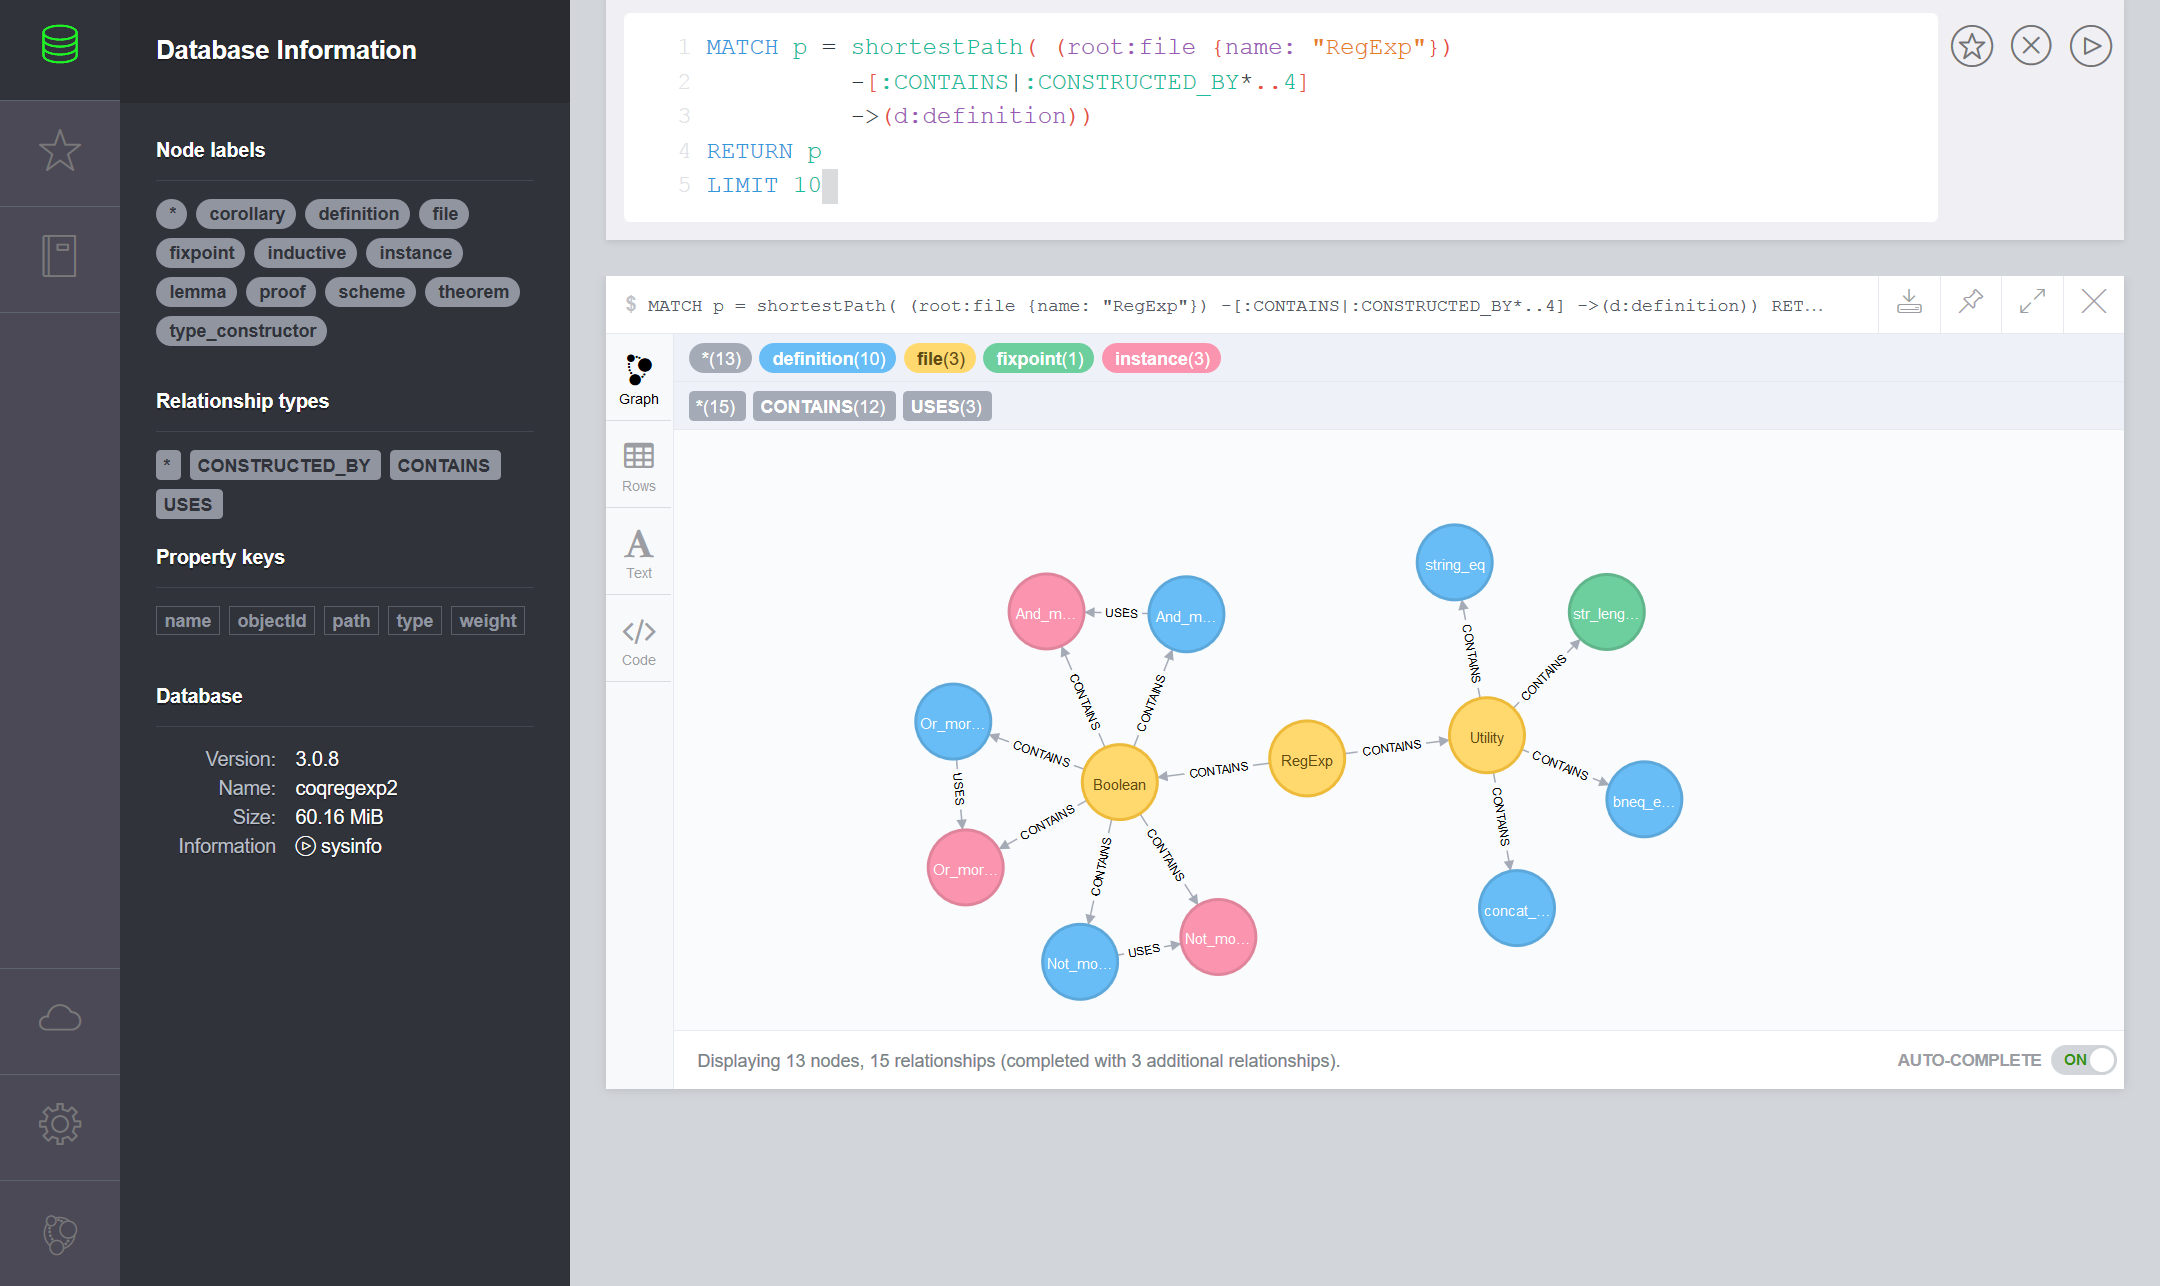
\includegraphics[width=\textwidth]{img/Neo4j_Browser.png}
\caption{Neo4j Interactive Browser. See Section~\ref{sec:neo4j} for a full
list of features.}\label{fig:neo4jbrowser}

\end{figure}

\section{Existing Tools for Neo4j}\label{subsec:existtoolsneo4j}

Neo4j features rich integration with many languages, libraries and tools.  Of
those, I found the following to be the most relevant and useful tools for
meeting this project requirements.

\subsection{APOC: Awesome Procedures on Cypher}

\href{http://github.com/neo4j-contrib/neo4j-apoc-procedures}{\emph{Awesome
Procedures on Cypher}, or \emph{APOC}} for short, is a community-maintained Java
plugin featuring several network-analysis algorithms, callable from within
Cypher itself.  Although there are other Cypher extension libraries (such as
MazeRunner), APOC is easy to install, well-documented, up-to-date and the most
comprehensive, and therefore the obvious choice as a foundation.

Thus, APOC helps step towards meeting the \emph{interaction} requirements for
this project by being easy to understand, flexible to use and extensible; it
even goes part-way towards meeting the \emph{computation} requirements.

\subsection{igraph}\label{subsubsec:neo4jtoolsigraph}

APOC's focus is on interacting with and combining different sorts and sources of
data and so lacks graph analysis functionality \emph{beyond} the basics. The
fact that it is implemented in Java adds to its limitations: it is not
well-suited to more intense analyses over large graphs of libraries and is
insufficient to \emph{fully} meet the \emph{computation} requirements of this
project.

For such tasks, \href{http://www.igraph.org}{igraph} is ideal: it is described
on its website as a \emph{collection of network analysis tools, with the
emphasis on efficiency, portability and ease of use}. Written in C/C++ (with
bindings for R and Python), igraph offers a \emph{comprehensive} set of graph
algorithms without sacrificing on performance. Some of these algorithms and
their uses are described in Subsection~\ref{subsec:igraphalg}.

Although igraph is not as easy to interact with  as APOC, the extra capabilities
it provided were indispensable towards achieving the \emph{computation}
requirements of a core library of good defaults.

\subsection{igraph Algorithms}\label{subsec:igraphalg}

igraph offers a comprehensive set of network-analysis algorithms. Becoming
familiar with these was a challenge and I spent several hours reading Newman's
\emph{Networks}~\cite{newman2008} in order to understand and use them correctly.
Network-analysis typically centres around two broad classes of measures:
centrality and community detection; both of which are described next.

\subsubsection{Centrality}

\emph{Centrality} measures offer a way to characterise a node's \emph{importance}.

\textbf{Betweenness} centrality is a measure based on shortest paths. For each
node ($v$), the fraction of shortest paths (from source $s$ to target $t$,
$\sigma_{st}$) which pass through it ($\sigma_{st}\left(v\right)$) is its
betweenness centrality. When applied to mathematical theories, how
``unavoidable'' a given object is for the results which mention
it.~\cite{freeman1977}

\begin{equation}
  g\left(v\right) = \sum_{s \neq v \neq t} \frac{\sigma_{st}\left(v\right)}{\sigma_{st}}
\end{equation}

\textbf{Closeness} centrality is a measure also based on shortest paths. For
each node, the sum of the length of all shortest paths to every other node is
its closeness centrality. In a directed, dependency graph of mathematical
theories, this corresponds to how ``foundational'' a node is. It is typically
calculated as the reciprocal of \emph{farness} ($\sum_{y}d\left(y,x\right)$),
scaled by the number of nodes in the graph ($N$) to allow comparisons with
graphs of different sizes.~\cite{bavelas1950}

\begin{equation}
  C\left(x\right) = \frac{N}{\sum_{y}d\left(y,x\right)}
\end{equation}

\textbf{PageRank} is a variant of \textbf{eigenvector} centrality.  For an
adjacency matrix $\mathbf{A}$, the v\textsuperscript{th} component of the
eigenvector $\mathbf{x}$ (whose entries must all be non-negative, corresponding
to the greatest eigenvalue $\lambda$) is the v\textsuperscript{th} node's
\emph{relative, eigenvector} centrality. Normalising the eigenvector provides
the \emph{absolute eigenvector} centralities.~\cite{newman2008}

The principle behind such a measure is that connections to high-ranking nodes
contribute more to a node's rank than connections to low-ranking nodes.  As
such, for mathematical theories, it is like a \emph{weighted
in-degree/number-of-uses} which takes into account the importance of the nodes
which is using a given type, proof or definition.

PageRank is similar; we want a vector $\mathbf{r}$ that satisfies
equation~\ref{eqn:pagerank}~\cite{page1999} instead of the equation $\mathbf{Ar}
= \lambda\mathbf{r}$ (for number of nodes $N$, random-jump probability $1-d$ and
stochastic adjacency matrix $\mathbf{L}$. Hence, it can be viewed as the
probability of a randomly-perusing mathematician coming across a given proof or
definition on a first reading.

\begin{equation}~\label{eqn:pagerank}
  \mathbf{r} = \frac{\left(1-d\right)}{N} \mathbf{1} + d\mathbf{Lr}
\end{equation}

\subsubsection{Community Detection}

Complex networks can exhibit community structure; that is, the graph can be
(roughly) divided into sparsely-connected, dense groups. Although mathematical
theories are often divided into sections, chapters and books, the following
algorithms provide scope for re-evaluating these groupings.

\textbf{Label propagation} is a simple, near linear time method for
determining which community a node belongs to. Each node starts with a unique
label, after which, on successive iterations, it adopts the label held by most
of its neighbours, until a consensus is reached. This whole procedure is
repeated a few times and an aggregate result constitutes the
output.~\cite{raghavan2007}

\textbf{Edge betweenness} (like betweenness centrality), is also based on
shortest paths, with the idea that edges separating communities are likely to
have high edge betweenness (since all shortest paths must pass through them).
Removing the edge with the greatest betweenness value and re-computing over the
remaining edges successively will result in a rooted tree, a hierarchical map
(called a dendrogram) where the root represents the whole graph and the leaves
represent individual nodes.~\cite{newman2004}

\textbf{Modularity} is a measure of how well network can be divided.  Formally,
it is the fraction of edges that fall within a given grouping (across the whole
graph) minus the expected number of those which could have fallen within the
group by chance (and so is a real number between $-0.5$ and $1$). Calculating
this in an optimal manner is an NP-complete problem, and so I used a fast and
greedy version of the algorithm instead.~\cite{clauset2004}

\subsection{visNetwork}

There exist \emph{several} visualisation programs for Neo4j; however, many are
for commercial, industrial use and offer the features/complexity (and pricing)
to match. All tools that offer live visualisation with built-in Cypher query
execution (e.g. KeyLines, TomSawyer, Linkurious) are proprietary, require a fee
to use and offer more granularity than I needed. Offline (and open-source)
solutions (which require data to be exported in some manner before
visualisation) such as Gephi or Alchemy.js offer similarly many features, but at
the cost of a steep learning curve. 

Ultimately, I chose
\href{http://datastorm-open.github.io/visNetwork}{visNetwork}, (an R library
exporting to JavaScript which can be rendered inside a browser) because it was
simple to use and easy to integrate with the rest of this project.

\subsection{R}\label{subsec:R}

\href{http://www.r-project.org}{R is a statistics-oriented programming
language}, part of the Free Software Foundation's GNU project. It is relevant for
this project because it offers an easy way to tie together Neo4j (through
official bindings), igraph and visNetwork.

To take advantage of this convenience, I had to learn R for this project. This
was not too difficult because R is a well-documented, relatively easy language
to pick-up.

\newpage
\section{Summary}

In this chapter, I gave a detailed account of how I planned this project. At the
start, I mentioned the choice of development methodology (spiral) and
development tools I used (Git, GitHub and Travis-CI). Following that, I
presented and explained the requirements this project should meet for modelling,
interacting with and analysing Coq libraries. From there, I stated how the
choice of technologies was dictated by the decision to use Coq and Neo4j.

I then elaborated on my starting point for this project. I gave a description of
Coq, its uses and explained why (complexity and poor documentation) it is a
difficult system to work with. I also compared existing tools that aim to help a
user understand a Coq library (coqdoc, coqdep, CoqSerAPI and dpdgraph) against
this project's requirements and showed that although none satisfied all the
requirements, dpdgraph provided a platform (albeit limited) to build upon.

Similarly, I gave a description of Neo4j and some of its plugins (APOC, igraph
and visNetwork) and explained their features, advantages, disadvantages in
relation to which of the project requirements they met. I discussed how I needed
to learn the R programming language to tie together Neo4j, igraph and visNetwork
in order to meet this project's interacting and computing requirements.
